\documentclass[11pt,a4paper,twocolumns]{article}
\usepackage[all]{xy}
\usepackage{pdftricks}
\usepackage{epsfig}
\usepackage{lipsum}
\usepackage{float}
\usepackage{verbatim}
\usepackage{geometry}
\usepackage{graphicx}
\usepackage{color}
\usepackage{epic}
\usepackage{eepic}
\usepackage{fontspec}
\usepackage[dvipdfm,a4paper,CJKbookmarks,bookmarks=true,bookmarksopen=true]{hyperref}
\begin{psinputs}
\usepackage{color}
\usepackage{pstcol}
\usepackage{pstricks}
\usepackage{pst-plot}
\usepackage{pst-tree}
\usepackage{pst-eps}
\usepackage{multido}
\usepackage{pst-node}
\usepackage{pst-eps}
\end{psinputs}
\definecolor{darkblue}{RGB}{0,0,128}
\hypersetup{
    pdftitle={CFT Minicomputer Programming Guide},
    pdfauthor={Alexios Chouchoulas},
    pdfkeywords={},
    bookmarksnumbered,
    pagebackref=true,
    breaklinks=true,
%    pdfview=FitH,       % Or try pdfstartview={FitV}, This lead to uncorrect bookmarks
    urlcolor=darkblue,
    colorlinks=true,
    citecolor=blue,          %citeref's color
    linkcolor=blue,
        }
% Fonts
%\defaultfontfeatures{Mapping=tex-text}
\setmainfont{Minion Pro}
\setsansfont{Myriad Pro}
\setmonofont[]{Inconsolata}

%\renewcommand{\rmdefault}{put}

\geometry{a4paper, hoffset=0in, voffset=-.25in, left=1.5cm, right=1.5cm,
  top=2.5cm, bottom=2.5cm}
\sloppy

% Use hyperlinking when renderind PDFs
\newcommand{\cf}[2][section]{\hyperref[#2]{#1 \ref*{#2} (p.~\pageref*{#2})}}
\newcommand{\npcf}[2][section]{\hyperref[#2]{#1 \ref*{#2}}}
\newcommand{\appcf}[1]{\cf[appendix]{#1}}
\newcommand{\ccf}[1]{\cf[chapter]{#1}}
\newcommand{\fcf}[1]{\cf[figure]{#1}}
\newcommand{\tcf}[1]{\cf[table]{#1}}
\newcommand{\ecf}[1]{\cf[equation]{#1}}
\newcommand{\algcf}[1]{\cf[algorithm]{#1}}
\newcommand{\npappcf}[1]{\npcf[appendix]{#1}}
\newcommand{\npccf}[1]{\npcf[chapter]{#1}}
\newcommand{\npfcf}[1]{\npcf[figure]{#1}}
\newcommand{\nptcf}[1]{\npcf[table]{#1}}
\newcommand{\npecf}[1]{\npcf[equation]{#1}}
\newcommand{\npalgcf}[1]{\npcf[algorithm]{#1}}

\setlength\columnsep{7mm}

\newcommand\hyperemail[1]{\sf\href{mailto:#1}{#1}}
\newcommand\link[1]{\sf\href{http://#1}{#1}}

\newcommand\register[1]{\textsf{#1}}
\newcommand\A{\register{AC}}
\newcommand\Lreg{\register{L}}
\newcommand\Ireg{\register{I}}
\newcommand\MAR{\register{AR}}
\newcommand\DR{\register{DR}}
\newcommand\PC{\register{PC}}
\newcommand\IR{\register{IR}}


\begin{document}
\thispagestyle{empty}
\pagestyle{plain}
\twocolumn[
\centering

\includegraphics{figs/cft-logo-v1.pdf}\vspace{2em}\\
{\LARGE\bf CFT Minicomputer Programming Guide}
\vspace{10pt}

{\Large Alexios Chouchoulas}\\\vspace{5pt}
{\large \hyperemail{alexios@bedroomlan.org}}

\vspace{20pt}

\begin{minipage}{.75\textwidth}
  \begin{abstract}
    \small
    
  This document discusses the architecture of the CFT computer from a
  programmer's perspective. The CFT is a solid-state, 16-bit,
  microcoded architecture reminiscent, among others, of the DEC
  PDP-8. The computer incorporates a 16-bit word width with separate
  memory and input/output addressing spaces and a minimal, orthogonal
  instruction set that is still particularly versatile. The design
  includes separate internal (processor) and external (peripheral)
  buses and is extensible both via processor extensions and
  peripherals.

  A brief explanation of the architecture is provided, along with a
  discussion of its programming model, instruction set, and
  limitations. Short examples of CFT Assembly code are provided, along
  with a complete opcode table with semantics and timing information.
    
  \end{abstract}
  
  \section*{History of Changes}
  \small

  {\bf 2011-10-10} First draft compiled from notes, hardware description
  and schematics.

  {\bf 2011-10-18} Fixed hexadecimal opcode of macro {\tt ING} in the
  instruction table. Corrected minor semantic and typesetting errors.
  
  \vspace{5ex}
  
\end{minipage}
] % End of \twocolumn
\section{Introduction}

  This document discusses the architecture of the CFT computer from a
  programmer's perspective. The CFT is a solid-state, 16-bit
  architecture reminiscent, among others, of the DEC
  PDP-8.\footnote{Newer versions of this document and additional
    documentation and downloads may be found at the following URL:\\
    \link{www.bedroomlan.org/hardware/cft}.}

  The computer incorporates a 16-bit word, 65,536 words of addressable
  main memory and 65,536 words of input/output (I/O) space.

  Instructions are 16-bits. There are seven registers and an simple,
  orthogonal instruction set. The computer is able to initialise
  itself without operator intervention using read-only ROM and a
  hardwired, turn-key bootstrap address. Communication to the outside
  world is attained using an interrupt facility, as part of an
  expansion bus that connects to main memory and peripherals. An
  autoindexing feature allows for very tightly coded looping
  structures.

  The design is microcoded for ease of upgrading.

\section{Architecture}

The CFT is a Von Neumann architecture stored program computer. Data is
primarily manipulated in memory, using the systems' single
general-purpose register as an intermediate. The design is such that
up to 1,024 general purpose registers may be accessed at any time. The
computer is completely solid-state, implemented using modern 74xxx
integrated circuits and some LSI memory.

The computer is microcoded. This simplifies upgrading and patching the
architecture to provide new features. Microcode consists of a number
of microprograms, each handling one CFT major state or
instruction. Each microprogram consists of up to 16 24-bit
microinstructions which operate directly the various physical units in
the computer.

The entire architecture is built around a 16-bit word. All data and
instructions is stored in 16-bit quantities, and all registers except
two are 16 bits wide. This allows programs and data to share the same
16-bit memory, and also makes programming significantly easier. An
rational, orthogonal instruction set with 15 main instructions and a
number of sub-instructions allows for ease of programming, yet
significant versatility.

The computer has separate address spaces for memory and input/output
devices, allowing the two to be kept separate. Through microcode
alterations additional wait states may be introduced for I/O, while
leaving memory accesses fast. This also allows processor extensions to
be built in I/O space, such as multiplication and division units,
novel instructions, et cetera.

\subsection{Word Size}

The word size is 16 bits. There are no facilities for accessing
quantities smaller than one word, and no single-instruction facilities
for accessing quantities longer than one word.

In this context, one kiloword (KWord) is $2^{10}$ or 1,024 kilowords.

\subsection{Data Types}

CFT defines a single data type: a 16-bit unsigned integer,
i.e. integers in the range 0–65,535. There are no instructions
explicitly intended to handle signed numbers, but two's complement
operations may still be performed and the hardware has been designed
to make this easier.

\subsection{Addressing}

The CFT architecture can address up to 64~KWords of memory, plus up to
64~KWords of I/O space\footnote{Although, for practical reasons, 1
  KWord of I/O space is more readily available.}.

\subsubsection{Memory Space}

Main memory is split up into 64 {\em pages\/}, each 1 KWord in
size. Instructions usually reference memory addresses relative to the
page they are executing in.

The first page, Page Zero, is given special treatment by the
instruction set. If bit 10 (starting at zero) of an instruction is
clear, addresses in Page Zero may be accessed. This is the fastest and
most convenient way of accessing memory beyond the current page. As
such, Page Zero is always used for system variables, constants and
other data that must be globally accessible.

The 128 words in Zero Page addresses {\tt 0080-00FF} (inclusive) are
so-called Autoindex registers. Using the Autoindex addressing mode,
each time one of these addresses is referenced, it is automatically
incremented by one. This allows loops to be coded very tightly, with
index register increments happening at the microcode level.

\begin{figure}[bt]
  \centering
  \begin{tabular}{cl}
    {\tt 0000} & {\tt SUBRET} — return address for last {\tt JSR}.\\
    {\tt 0001} & {\tt TRAPRET} — return address for last {\tt TRAP}\\
    {\tt 0002} & {\tt ISRRET} — return address for last ISR.\\
    {\tt 0080} & {\tt IR0} — first autoindex register.\\
    {\tt 00FF} & {\tt IR7F} — last (128th) autoindex register.\\
    $\vdots$ & $\vdots$ \\
    {\tt 03FF} & Last word of Page Zero.\\
    {\tt 1000} & First word of Page 1.\\
    $\vdots$ & $\vdots$ \\
    {\tt 8000} & First word of Page 32.\\
    $\vdots$ & $\vdots$ \\
    {\tt FC00} & First word of Page 63.\\
    {\tt FFF0} & Boot/reset address.\\
    {\tt FFF8} & Interrupt service routine.\\
    {\tt FFFF} & Highest memory address.\\
  \end{tabular}
  \caption{\label{fig-mm}Memory map of the CFT CPU's memory space.}
\end{figure}

\subsubsection{I/O Space}

Although there are 64 KWords of I/O space, this is limited by
practical limitations: Only the first 1,024 I/O addresses may be
accessed from anywhere in memory space. Due to page-relative
addressing, accessing the rest of the I/O space is mostly convenient
via indirect addressing. For speed and ease of use, most I/O devices
will thus occupy the first KWord of address space. Page-relative
addressing is discussed in detail in \cf{sec-pagerel}.

\subsection{Registers}

\begin{figure}[tb]
  \centering
  \begin{pdfpic}
    \begin{pspicture}(-1,-1)(8,7)
      \newrgbcolor{vlgrey}{1 1 1}
      \rput(0,0){
        {\psset{linewidth=3\pslinewidth}\psframe(7.5,0)(8,0.75)}
        \psset{linewidth=0.33\pslinewidth}
        \rput[B](7.75,0.27){I}
        \rput[tl](7.5,-0.1){\footnotesize 1}
        \rput[tr](8,-0.1){\footnotesize 0}
      }
      \rput(0,1.25){
        {\psset{linewidth=3\pslinewidth}\psframe(7.5,0)(8,0.75)}
        \psset{linewidth=0.33\pslinewidth}
        \rput[B](7.75,0.27){L}
        \rput[tl](7.5,-0.1){\footnotesize 1}
        \rput[tr](8,-0.1){\footnotesize 0}
      }
      \rput(0,2.5){
        {\psset{linewidth=3\pslinewidth}\psframe[fillstyle=solid,fillcolor=vlgrey](0,0)(8,0.75)}
        \psset{linewidth=0.33\pslinewidth}
        \rput[B](4,0.27){MAR}
        \rput[tl](0,-0.1){\footnotesize 15}
        \rput[tr](8,-0.1){\footnotesize 0}
      }
      \rput(0,3.75){
        {\psset{linewidth=3\pslinewidth}\psframe[fillstyle=solid,fillcolor=vlgrey](0,0)(8,0.75)}
        \psset{linewidth=0.33\pslinewidth}
        \rput[B](4,0.27){IR}
        \rput[tl](0,-0.1){\footnotesize 15}
        \rput[tr](8,-0.1){\footnotesize 0}
      }
      \rput(0,5){
        {\psset{linewidth=3\pslinewidth}\psframe[fillstyle=solid,fillcolor=vlgrey](0,0)(8,0.75)}
        \psset{linewidth=0.33\pslinewidth}
        \rput[B](4,0.27){DR}
        \rput[tl](0,-0.1){\footnotesize 15}
        \rput[tr](8,-0.1){\footnotesize 0}
      }
      \rput(0,6.25){
        {\psset{linewidth=3\pslinewidth}\psframe[fillstyle=solid,fillcolor=vlgrey](0,0)(8,0.75)}
        \psset{linewidth=0.33\pslinewidth}
        \rput[B](4,0.27){PC}
        \rput[tl](0,-0.1){\footnotesize 15}
        \rput[tr](8,-0.1){\footnotesize 0}
      }
      \rput(0,7.5){
        {\psset{linewidth=3\pslinewidth}\psframe(0,0)(8,0.75)}
        \psset{linewidth=0.33\pslinewidth}
        \rput[B](4,0.27){A}
        \rput[tl](0,-0.1){\footnotesize 15}
        \rput[tr](8,-0.1){\footnotesize 0}
      }
    \end{pspicture}
  \end{pdfpic}
  \caption{\label{fig-rf}Full Register file. Only the \A, \Lreg\  and \Ireg\  registers are made directly accessible to the user.}
\end{figure}

There are seven registers in the CFT architecture.

\subsubsection{Accumulator (\A)}

The Accumulator (\A) is a 16 bit register. It is the only 16-bit
register directly and fully accessible via the instruction set and the
one almost all instructions operate on.

\subsubsection{Link Register (\Lreg)}

The Link Register (\Lreg) is a single-bit register. It is used as a carry
or overflow bit during arithmetic and as the 17th bit during roll
instructions. It may be used as a generic flag by user programs.

\subsubsection{Program Counter (\PC)}

The Program Counter is a 16-bit register. It contains the address of
the next instruction to be executed. It may not be read, but can be
indirectly affected by way of skips, jumps, subroutine calls, traps,
and interrupts.

\subsubsection{Interrupt Register (\Ireg)}

This 1-bit register controls the computer's behaviour on detecting an
interrupt request. The register may be manipulated by the user to
allow or mask interrupts.

\subsubsection{Instruction Register (\IR)}

The Instruction Register (\IR) holds the instruction currently being
executed. It is 16 bits wide and is used internally only. There is no
way to access it.

\subsubsection{Memory Address Register (\MAR)}

The Memory Address Register (\MAR) is a 16-bit register that buffers
most addresses that are put out on the CFT address bus. The exception
is indirect addressing, which uses the Data Register. It cannot be
accessed by the user.

\subsubsection{Data Register (\DR)}

The Data Register (\DR) is a 16-bit register used internally by the CFT
to buffer addresses during indirect addressing. Like the \MAR, the \DR
cannot be accessed by the user.

\subsection{Instruction Format}
\label{sec-if}

\begin{figure}[tb]
  \centering
  \begin{pdfpic}
    \begin{pspicture}(-1,-1)(8,1)
      \psset{linewidth=3\pslinewidth}
      \psframe(0,0)(8,0.75)
      \psset{linewidth=0.33\pslinewidth}
      \psline{-}(2,-0.1)(2,0.75)
      \psline{-}(2.5,-0.1)(2.5,0.75)
      \psline{-}(3,-0.1)(3,0.75)
      \rput[B](1,0.27){Opcode}
      \rput[B](2.25,0.27){I}
      \rput[B](2.75,0.27){R}
      \rput[B](5.5,0.27){Operand}
      \rput[tl](0,-0.1){\footnotesize 15}
      \rput[tl](3.1,-0.1){\footnotesize 9}
      \rput[tr](2.9,-0.1){\footnotesize 10}
      \rput[tr](2.4,-0.1){\footnotesize 11}
      \rput[tr](1.9,-0.1){\footnotesize 12}
      \rput[tr](8,-0.1){\footnotesize 0}
    \end{pspicture}
  \end{pdfpic}
  \caption{\label{fig-if}Instruction Format of the CFT architecture.}
\end{figure}

The CFT computer uses a single instruction format. All instructions are exactly
16 bits wide and comprise the same fields, as shown in~\fcf{fig-if}. Each
instruction contains four fields. From most to least significant, they are:

\begin{description}
\item{\bf The Instruction opcode (most significant 4 bits)}. This
  field identifies the instruction to be performed.
\item{\bf The Indirection mode (1 bit)}. Depending on the instruction,
  this bit selects between the literal and direct, or the direct and
  indirect addressing mode.
\item{\bf The Register Mode (1 bit)}. This bit controls whether
  addresses and literals are relative to the current page, or relative
  to page zero (the register page).
\item{\bf The Operand or address offset (least significant 10
  bits)}. This allows only ten bits of literals or addresses to be
  specified in an instruction. The most significant six bits are
  filled in from one of two sources as follows:
  \begin{itemize}
  \item If the Register Mode bit is set (1), the six most significant bits
    of the \PC\ register are used. This is page-relative addressing.
  \item If the Register Mode bit is clear (0), the six most
    significant bits of the operand are zero. This is Register
    addressing, also known as Page-Zero addressing, since Page Zero is
    used for system registers.
  \end{itemize}
  This introduces a number of limitations, discussed in~\cf{sec-pagerel}.
\end{description}

\subsection{Page-Relative Limitations}
\label{sec-pagerel}

Unless the Register Mode (R) bit is enabled (field R in the
instruction equal to 0), an instruction at address {\tt addr} may only
access memory (and I/O) address between {\tt addr AND FC00} and {\tt
  (ADDR AND FC00) OR 3FF}. This introduces a number of limitations and
defines the programming style of CFT more than any other single
aspect of the design.

There are four obvious solutions to the limitation:

Subprograms need to store temporary data on the local page, or to use
special ‘scratch’ registers in Page Zero. Both addressing modes take
the same time to execute.

In the case of constants, the programmer can either limit themselves
to constants in the range {\tt 0000}–{\tt 03FF}, store commonly-used
large constants (such as -1, {\tt FFFF} and -2, {\tt FFFE}) in a Page
Zero constant table, or a combination of these techniques\footnote{A
  note for PDP-8 programmers: the CFT has a {\tt LI} (Load Immediate)
  instruction that can load the Accumulator with a 10-bit
  literal. This is considerably faster the the only PDP-8 alternative,
  constructing basic constants using microcoded instructions.}.

Special care needs to be taken for subprograms longer than 1,024
words. If code crosses a page boundary, references to any local data
will in fact refer to the same offset within the {\tt new\/} page, and
will of course be invalid.

The standard assembler issues a cross-page warning when using symbolic
names (labels) for such local data, which is a very good practice.

Jumps, subroutine calls and traps suffer from the same issue. Indirect
Register addressing is commonly used as a solution to this problem:
the address (vector) of the subprogram in question is stored in a Page
Zero location, and the jump is made using indirection. This has the
added benefit of allowing the vectors to be changed so that system
services may be overridden.

Perhaps the most significant limitation, however, is on the size of
the I/O address space. When performing page-relative I/O operations
({\tt IN}, {\tt OUT} and {\tt IOT}), the most significant six bits of
the I/O address will {\em still\/} be taken from the six most
significant bits of the \PC. Because of this, different I/O devices
will be accessed depending on the location of the program in
memory. There are two ways to avoid this: the primary one is to only
use 10 bits of I/O space. Either the R field in all I/O instructions
must be 0, or the hardware must decode only the 10 least significant
address lines\footnote{Thus providing six don't care bits, which is 64
  copies of every I/O device, one for every page.}, or a combination
of both. The secondary means of avoiding this issue is indirect
addressing. It is assumed that a mixture of these techniques will be
used in practice. Please refer to your system documentation for exact
details.

\subsection{Addressing Modes}

CFT instructions have two bits that modify how instructions treat the
operand field: the R (register) field, and the I (indirection)
field.

The R field controls how the six most significant bits of the operand
are derived, as described in~\cf{sec-if}.

The I field controls how the resultant operand is used. This depends
on the instruction.

Combined, there are up to four addressing modes per instruction. There
is also a fifth addressing mode, autoindex mode, which is selected for
specific memory addresses only. Each instruction supports five
addressing modes. 

Naturally, no instructions support all addressing modes. Depending on
the nature of the instruction, either literal and direct modes, or
direct and indirect modes are used. There also some instructions in
which the addressing mode does not apply. This is indicated as
‘special’ mode.

The addressing modes are as follows:

\begin{itemize}
  \item Immediate.
  \item Immediate page-relative.
  \item Direct register.
  \item Direct page-relative.
  \item Indirect register.
  \item Indirect page-relative.
  \item Indirect autoindex.
  \item Special.
\end{itemize}

\subsubsection{Immediate Mode}

When using applicable instructions with R=0 and I=0, the value field
in the instruction is used as the least significant 10 bits of a
literal value. The most significant six bits are zero. This allows
literal values in the range {\tt 0000–03FF} to be specified.

For example, executing the Load Immediate (LI R) instruction {\tt LI R
  0350} will set \A={\tt 0350}.

\subsubsection{Immediate Page-Relative Mode}

When using applicable instructions with with R=1 and I=0, the value
field in the instruction is used as the least significant 10 bits of a
literal value. The most significant six bits of the \PC\  are used as the
most significant six bits of that value. This allows addresses in the
current page to be specified.

For example, executing the Load Address (LIA) instruction {\tt LIA
  0042} at address {\tt 2130} will set \A={\tt 2042}.

\subsubsection{Direct Register Mode}

When using applicable instructions with R=0 and I=0, the value field
in the instruction is used as the least significant 10 bits of a
memory or I/O address. The most significant six bits are zero. This
allows Page Zero registers and I/O devices to be addressed.

For example, executing the Load instruction {\tt LOAD R 0010}
instruction will load the contents of address {\tt 0010} into \A.

\subsubsection{Direct Page-Relative Mode}

When using applicable instructions with R=1 and I=0, the value field
in the instruction is used to construct an address which is used
directly to reference a value in memory or I/O space. This is the most
commonly used addressing mode.

For example, executing the Store instruction {\tt STORE 0010} at
address {\tt 8514} will write the contents of \A\  onto memory address
{\tt 8410}.

\subsubsection{Indirect Register Mode}

When using applicable instructions with R=0 and I=1, the value field
in the instruction is used to construct an address. The 16-bit value
{\em at that address in memory\/} is used to reference memory or I/O
space.

For example, executing the LOAD instruction {\tt LOAD I 009A} will
read into the \DR register a 16-bit value from memory location {\tt
  009A}. \A\  will then be loaded with the value of the address in
memory stored in \DR.

\subsubsection{Indirect Mode}

When using applicable instructions with R=1 and I=1, the value field
in the instruction is used to construct an address. The 16-bit value
at that address in memory is used to reference memory or I/O space.

For example, executing the LOAD instruction {\tt LOAD I 009A} at
address {\tt 1234} will read into the Data Register a 16-bit value
from memory location {\tt 109A}. That number is treated as the address
in memory to be read into \A.

\subsubsection{Autoindex Mode}

Autoindex mode operates like indirect mode above, but the memory
location indicated in the instruction field is incremented after being
used. Autoindex mode cannot be selected directly. It is automatically
enabled for addresses in the range {\tt 0080}–{\tt 00FF}. The value of the R
field is immaterial, only the address is examined.

For example, executing the LOAD instruction {\tt LOAD I R 009A} will
read into the \DR register a 16-bit value from memory location {\tt
  109A}. That number is used as the address in memory to be read
into \A, then incremented by one and written back to location {\tt
  009A}.

If the instruction were {\tt LOAD I 009A} and it executed at address
{\tt 0003}, the result would have been the same.

\subsection{Operating States}

The CFT CPU has four major operating states: initialisation, interrupt,
operation and waiting.

\subsubsection{Initialisation}

When the computer initialises via a system reset or initial boot, it
sets \PC\  to the boot address {\tt FFF0} and clears the \Ireg\  register
to disallow interrupts. All other registers are undefined and may
contain arbitrary values — boot code should initialise any register
necessary for its operation. Normal operation is then resumed.

\subsubsection{Interrupt}

When the computer encounters an interrupt, and if the \Ireg\ register is {\tt
  1} (allowing interrupts), the event is buffered in a minor state
register. When the currently executing instruction is completed, the
\Ireg\ register is cleared to disable further interrupts and the current value
of the \PC\ is written to memory address {\tt 0002}. Finally, the \PC\ is
loaded with the value {\tt FFF8}, which is the address of the Interrupt Service
Routine (ISR). Normal operation is then resumed.

\subsubsection{Operation}

During normal fetch-execute operation, the computer's microcode
fetches instructions from main memory address indicated by \PC,
increments the \PC, then executes the fetched instructions. This is the
mode the computer spends most of its time in.

\subsubsection{Wait}

On occasion, external slow hardware or the operator's console may halt
the processor's clocks. In this state, the sequencer does not work
through the microcode and the computer does not operate.

This mode may be entered at any time. The operator's console allows it
to be entered either inside a microprogram, or immediately before the
fetch part.

The Wait state is transient: as soon as the appropriate signals are
de-asserted by the hardware, the previous state resumes.

\section{Instruction Set Reference}

The first edition of the CFT microcode allowed for fourteen different
instructions. The second edition added the {\tt IOT} instruction,
which makes for fifteen mutually orthogonal instructions:

\begin{itemize}
\item {\tt TRAP}: save the \PC\ and jump to the specified location. Used for operating system services.
\item {\tt IOT}: new in version 2.0 of the microcode. Writes to a specified output device, then reads a result back from it. Used to implement computer extensions via I/O-addressable extension units.
\item {\tt LOAD}: load from memory.
\item {\tt STORE}: write to memory.
\item {\tt IN}: read from an input device.
\item {\tt OUT}: write to an output device.
\item {\tt JMP}: unconditional jump to the specified location.
\item {\tt JSR}: save the \PC\ and jump unconditionally to the specified location.
\item {\tt ADD}: load from memory and add to the accumulator.
\item {\tt AND}: load from memory and perform a bitwise AND with the value in the accumulator.
\item {\tt OR}: load from memory and perform a bitwise OR with the value in the accumulator.
\item {\tt XOR}: load from memory and perform a bitwise exclusive OR with the value in the accumulator.
\item {\tt OP1}: minor operations, group one.
\item {\tt OP2}: minor operations, group two.
\item {\tt LIA}: load accumulator with literal value or address.
\end{itemize}

To simplify understanding of the instruction set, opcode mnemonics are
used rather than actual machine code. In many cases, the notation used
is that of the Standard CFT Assembly language which merits some
description. This is not a full definition of CFT Assembly language,
merely enough of it to facilitate discussing the instruction set in
a more human-readable form.

CFT Assemblers parse lexical tokens denoting either symbolic
instruction names or hexadecimal numbers. Symbols are converted to
numbers using symbol tables. The resultant numbers, which must be 16
bits in width, are ORred together to form an instruction\footnote{One
  exception is the {\tt R} symbol, which {\em clears\/} bit 10 of the
  instruction to turn on Page Zero/register addressing modes. In
  practice, this is not actually an exception. After assembling an
  instruction, however, the Assembler performs an {\tt XOR} with the
  hexadecimal value {\tt 0400} (complementing bit 10), which allows
  the bitwise Or semantics to work for everything, including the R
  flag, and the resultant code to run as expected.}.

This provides great simplicity and generality at the expense of making
the code slightly less readable from a modern Assembly
perspective\footnote{PDP-8 Assembly programmers will feel right at
  home, though.}).

Anything after the first semicolon ({\tt ;}) on a line is considered a
comment and ignored.

A brief example of CFT Assembly language can be found in~\fcf{fig-asm}.

\begin{figure}
\small
\begin{verbatim}
LOAD 0000     ; Load direct
LOAD I 0342   ; Load indirect
0342 I LOAD   ; Valid, but against conventions.
LOAD I R 007F ; Load zero page and indirect
LOAD I R 0080 ; Load, autoindexing
IN R PANEL 0  ; Read panel switches
CLL RBL       ; Shift left one bit
HALT          ; Halt the system
\end{verbatim}
\caption{\label{fig-asm}Examples of CFT instructions in Assembly language .}
\end{figure}

\subsection{Memory}

The following instructions operate on memory space.

\subsubsection{{\tt LOAD} — Load Accumulator}
\label{sec-load}

Load a word from memory into \A. Direct, indirect and autoindex modes are available.

\subsubsection{{\tt STORE} — Store Accumulator}
\label{sec-store}

Write \A\ to the specified memory location. Direct, indirect and autoindex modes are available.

\subsection{I/O}

The following instructions operate on I/O space.

\subsubsection{{\tt IN} — Read from I/O Device}
\label{sec-in}

Read a word from I/O space into \A. Direct, Indirect and autoindex
modes are available. {\tt IN} instructions may have additional
side-effects that depend on the peripheral being addressed.

\subsubsection{{\tt OUT} — Write to I/O Device}
\label{sec-out}

Write the contents of \A\ to the specified I/O space address. Direct,
Indirect and autoindex modes are available. {\tt OUT} instructions
almost always have side-effects that depend on the peripheral being
addressed.

\subsubsection{{\tt IOT} — I/O Transaction}
\label{sec-iot}

Implements a processor extension. The {\tt IOT} instruction writes A
to I/O space, the reads A back from the same address. The I/O-mapped
processor extension can introduce wait states at the end of the I/O
space read cycle, in order to get more time to perform its
task. Direct, Indirect and autoindex modes are available.

\subsection{Arithmetic and Logic}

The following instructions perform common arithmetic and logic operations.

\subsubsection{{\tt ADD} — Add to Accumulator}
\label{sec-add}

Read a word from memory and add it to \A. If the addition results in a
carry-out, \Lreg\  is toggled. Direct, Indirect and autoindex modes are
available.

\subsubsection{{\tt AND} — Bitwise And with Accumulator}
\label{sec-and}

Read a word from memory and perform a bitwise AND operation with A. Direct, Indirect and autoindex
modes are available.

\subsubsection{{\tt OR} — Bitwise Or with Accumulator}
\label{sec-or}

Read a word from memory and perform a bitwise OR operation with A. Direct, Indirect and autoindex
modes are available.

\subsubsection{{\tt XOR} — Bitwise Exclusive OR with Accumulator}
\label{sec-xor}

Read a word from memory and perform a bitwise XOR operation with A. Direct, Indirect and autoindex
modes are available.

\subsection{Flow Control}

The following instructions implement flow control via modification of the \PC\ register.

\subsubsection{{\tt TRAP} — Jump to System Service}
\label{sec-trap}

Writes the value of the \PC to memory location {\tt 0001}, then sets
the \PC to the address specified in the instruction. Direct, Indirect
and autoindex modes are available.

\subsubsection{{\tt JMP} — Jump to Address}
\label{sec-jmp}

Sets the \PC to the address specified in the instruction. Direct,
Indirect and autoindex modes are available.

\subsubsection{{\tt JSR} — Jump to Subroutine}
\label{sec-jsr}

Writes the value of the \PC to memory location {\tt 0000}, then sets
the \PC to the address specified in the instruction. Direct, Indirect
and autoindex modes are available.

\subsection{Specials}

These are operations that do not fit in the categories above.

\subsubsection{{\tt OP1} — Operations 1}
\label{sec-op1}

\begin{figure*}[tb]
  \centering
  
  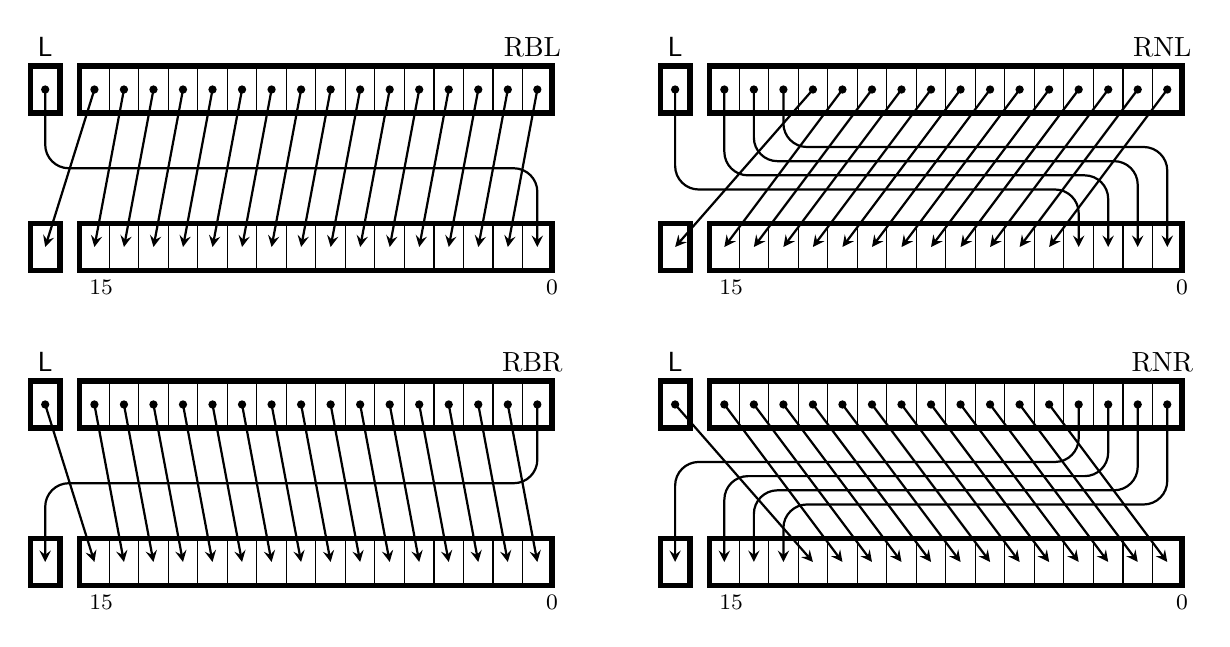
\begin{tikzpicture}
    \newcommand\xxroll[2]{
      \begin{scope}[#1]
        
        \foreach \x in {0, -2} {
          \begin{scope}[yshift=\x cm]
            \draw[line width=2pt](0,0) rectangle (6,0.6);
            \draw[line width=2pt](-0.25,0) rectangle (-0.625,0.6);
            \foreach \x in {0.375, 0.75, ..., 5.625} {
              \draw[thin] (\x cm, 0) -- (\x cm, 0.6cm);
            }
          \end{scope}
        }
        
        \fill (-0.4375, 0.3) circle (1.5pt);
        \foreach \x in { 0.1875, 0.5625, ..., 5.8125 } \fill (\x, 0.3) circle (1.5pt);
        \draw (5.75, 0.6) node[above] { \op{#2}};
        \draw (-0.4375, 0.6) node[above] { \Lreg };
        \draw (-0.1, 0.6) node[above right=0/0.25cm] { \Areg };
        \draw (6,-2) node[below] { \footnotesize 0 };
        \draw (0,-2) node[below right] { \footnotesize 15 };
      \end{scope}
    }

    % RBL
    \begin{scope}
      \xxroll{}{RBL}
      \draw[thick, -stealth] (.1875, 0.3) -- (-.4375, -1.7);
      \foreach \x in {0.1875, 0.5625, ..., 5.4375} {
        \draw[thick, -stealth] (\x + 0.375, 0.3) -- (\x, -1.7);
      }
      \draw[thick, -stealth, rounded corners=3mm] (-0.4375, 0.3) -- (-0.4375, -0.7) -- (5.8125, -0.7) -- (5.8125, -1.7);
    \end{scope}

    % RBR
    \begin{scope}[yshift=-4cm]
      \xxroll{}{RBR}
      \draw[thick, -stealth] (-0.4375, 0.3) -- (.1875, -1.7);
      \foreach \x in {0.1875, 0.5625, ..., 5.4375} {
        \draw[thick, -stealth] (\x, 0.3) -- (\x + 0.375, -1.7);
      }
      \draw[thick, -stealth, rounded corners=3mm] (5.8125, 0.3) -- (5.8125, -0.7) -- (-0.4375, -0.7) -- (-0.4375, -1.7);
    \end{scope}

    % RNL
    \begin{scope}[xshift=8cm]
      \xxroll{}{RNL}
      \begin{scope}[thick,-stealth]
        \draw (0.1875 + 3 * 0.375, 0.3) -- (-.4375, -1.7);
        \foreach \x in {4, ..., 15} {
          \draw (0.1875 + 0.375 * \x, 0.3) -- ++(-4 * 0.375, -2);
        }
        \begin{scope}[rounded corners=3mm]
          \draw (-.4375, 0.3) -- (-.4375, -.25 - .18 * 4) -- 
          ( 0.1875 + 0.375 * 12, -.25 - .18 * 4) -- (0.1875 + 0.375 * 12, -1.7);
          \draw (0.1875, 0.3) -- (0.1875, -.25 - .18 * 3) -- 
          ( 0.1875 + 0.375 * 13, -.25 - .18 * 3) -- (0.1875 + 0.375 * 13, -1.7);
          \draw (0.1875 + 0.375, 0.3) -- (0.1875 + 0.375, -.25 - .18 * 2) -- 
          ( 0.1875 + 0.375 * 14, -.25 - .18 * 2) -- (0.1875 + 0.375 * 14, -1.7);
          \draw (0.1875 + 0.375 * 2, 0.3) -- (0.1875 + 0.375 * 2, -.25 - .18) -- 
          ( 0.1875 + 0.375 * 15, -.25 - .18) -- (0.1875 + 0.375 * 15, -1.7);
        \end{scope}
      \end{scope}
    \end{scope}

    % RNR
    \begin{scope}[xshift=8cm, yshift=-4cm]
      \xxroll{}{RNR}
      \begin{scope}[thick,-stealth]
        \draw (-.4375, 0.3) -- (0.1875 + 3 * 0.375, -1.7);
        \foreach \x in {0, ..., 11} {
          \draw (0.1875 + 0.375 * \x, 0.3) -- ++(4 * 0.375, -2);
        }
        \begin{scope}[rounded corners=3mm]
          \draw (0.1875 + 0.375 * 12, 0.3) -- (0.1875 + 0.375 * 12, -.25 - .18 * 1) -- ( -.4375, -.25 - .18 * 1) -- (-.4375, -1.7);
          \draw (0.1875 + 0.375 * 13, 0.3) -- (0.1875 + 0.375 * 13, -.25 - .18 * 2) -- ( 0.1875, -.25 - .18 * 2) -- (0.1875, -1.7);
          \draw (0.1875 + 0.375 * 14, 0.3) -- (0.1875 + 0.375 * 14, -.25 - .18 * 3) -- ( 0.1875 + 0.375, -.25 - .18 * 3) -- (0.1875 + 0.375, -1.7);
          \draw (0.1875 + 0.375 * 15, 0.3) -- (0.1875 + 0.375 * 15, -.25 - .18 * 4) -- ( 0.1875 + 0.375 * 2, -.25 - .18 * 4) -- (0.1875 + 0.375 * 2, -1.7);
        \end{scope}
      \end{scope}
    \end{scope}
  \end{tikzpicture}

  \caption{\label{fig-roll}Roll Instructions.}
\end{figure*}

The {\tt OP1} instruction provides a number of minor operations, any
number of which may be performed in a preset order. This is very
similar to the PDP-8 ‘microcoded’ instructions.

The operand of the {\tt OP1} instruction is seen as a bitfield, where
set bits trigger a particular minor operation. The table below
outlines the possible operations that can be ORred together.

\vspace{1em}\noindent\begin{center}
\begin{tabular}{ll}
  Bitfield & {\tt OP1} Instruction \\\noalign{\smallskip}\hline\noalign{\smallskip}
  {\tt 1---------} & {\tt CLA} — Clear \A \\
  {\tt -1--------} & {\tt CLL} — Clear \Lreg \\
  {\tt --1-------} & {\tt NOT} — Complement \A \\
  {\tt ---1------} & {\tt INC} — Increment (\Lreg,\A) by one \\
  {\tt ----1-----} & {\tt CPL} — Complement \Lreg \\
  %{\tt -----1----} & {\em Reserved} \\
  %{\tt ------1---} & {\em Reserved} \\
  {\tt -------010} & {\tt RBL} — Roll Bit Left (\Lreg,\A) \\
  {\tt -------001} & {\tt RBR} — Roll Bit Right (\Lreg,\A) \\
  {\tt -------110} & {\tt RNL} — Roll Nybble Left (\Lreg,\A) \\
  {\tt -------101} & {\tt RNR} — Roll Nybble Right (\Lreg,\A) \\\noalign{\smallskip}\hline\noalign{\smallskip}
\end{tabular}
\end{center}\vspace{1em}

These operations is performed in the order in which they appear above,
from top to bottom. If no operations are specified, i.e. the
instruction is {\tt C000}, the instruction is effectively a NOP. The
four roll instructions are mutually exclusive. The notation (\Lreg,\A)
indicates that both \Lreg\ and \A\ are used together as a 17-bit
quantity, with \Lreg\ becoming the most significant bit.

To clear both A and L, the instruction would be {\tt OP1 CLA CLL}.

If the {\tt INC} instruction is issued when \A={\tt FFFF}, \Lreg\ is
toggled. As expected, \A\ becomes {\tt 0000}.

To calculate the two's complement of A {\tt OP1 NOT INC} (hexadecimal
instruction {\tt C300}) will first invert A, then increment it by
one. Note that {\tt OP1 INC NOT} has exactly the same result, as the
order in which minor operations are performed is fixed.

A binary left shift by one bit can be defined as {\tt OP1 CLL RBL}
({\tt C102}).

The standard Assembler defines many of these combinations of 
instructions as
convenient macros. When using these macros, specifying {\tt OP1} is
optional.

The exact operation of the four roll instructions is illustrated
in~\npfcf{fig-roll}.

\subsubsection{{\tt OP2} — Operations 2}
\label{sec-op2}

This instruction is very similar to the {\tt OP1} instruction. The
main feature of the {\tt OP2} instruction is skipping. Skip
instruction skip over the following instruction if the corresponding
condition is true. Conditions involve the A and L registers. The
following table lists the {\tt OP2} bitfield values that may be ORred
together.

\vspace{1em}\noindent\begin{center}
\begin{tabular}{ll}
  Bitfield & {\tt OP2} Instruction \\\noalign{\smallskip}\hline\noalign{\smallskip}
  {\tt ------01--} & {\tt SNA} — Skip if A negative (G1)\\
  {\tt ------0-1-} & {\tt SZA} — Skip if A zero (G1) \\
  {\tt ------0--1} & {\tt SSL} — Skip if L set (G1) \\
  {\tt ------1000} & {\tt SKIP} — Always skip (G2) \\
  {\tt ------11--} & {\tt SNN} — Skip if A non-negative (G2) \\
  {\tt ------1-1-} & {\tt SNZ} — Skip if A non-zero (G2) \\
  {\tt ------1--1} & {\tt SCL} — Skip if L clear (G2) \\
  {\tt ---1------} & {\tt CLA2} — Clear A \\
  {\tt ----1-----} & {\tt CLI} — Clear I flag \\
  {\tt -----1----} & {\tt STI} — Set I flag \\%
  \noalign{\smallskip}\hline\noalign{\smallskip}
\end{tabular}
\end{center}\vspace{1em}

There are two groups of branching instructions: G1 (bit 3 of the
instruction operand is {\tt 0}) and G2 (bit 3 of the instruction
operand is {\tt 1}). When G1 instructions {\tt SNA}, {\tt SZA} and
{\tt SSL} are specified together, the skip is performed when any of
the specified conditions hold (logical disjunction or Or). For example, the
instruction {\tt SZA SNA} is ‘skip if A less than or equal to zero’,
or ‘skip if A non-positive’ (which is the standard CFT Assembly macro
{\tt SNP}).

When G2 instructions are specified together, the skip is performed
when all of the specified conditions hold (logical conjunction or And). For
example, {\tt SNN SNZ} is ‘skip if A is non-zero and non-negative’, or
‘skip if A is positive’ (the standard Assembler macro for this is {\tt
  SPA}). The full set of combinations to check the value of A is as
follows:

\vspace{1em}\noindent\begin{center}
\begin{tabular}{lll}
  Instruction & Macro & Semantics \\\noalign{\smallskip}\hline\noalign{\smallskip}
  {\tt SNA }     &           & Skip if $\mbox{A} < 0$ \\
  {\tt SNA SZA } & {\tt SNP} & Skip if $\mbox{A} \leq 0$ \\
  {\tt SZA }     &           & Skip if $\mbox{A} = 0$ \\
  {\tt SNZ }     &           & Skip if $\mbox{A} \not= 0$ \\
  {\tt SNN }     &           & Skip if $\mbox{A} \geq 0$ \\
  {\tt SNN SNZ } & {\tt SPA} & Skip if $\mbox{A} > 0$ \\
  \noalign{\smallskip}\hline\noalign{\smallskip}
\end{tabular}
\end{center}\vspace{1em}

\subsubsection{{\tt LIA} — Load Immediate Address}
\label{sec-lia}
\label{sec-li}

Loads A with the literal value specified in the instruction. The
page-relative form of this instruction is used to load A with a
page-relative address.

When R=0, {\tt LIA} becomes the Load Immediate ({\tt LI}) instruction,
which can load a value in the range {\tt 0000}–{\tt 03FF} into A.

This instruction always operates in the Immediate addressing mode. The
value of the instruction I bit is {\em ignored}.

\subsection{Standard Macros}
\subsubsection{{\tt RET} — Return from Subroutine}

This is defined as {\tt JMP I R 0000}. It jumps to the return address
saved by the {\tt JSR} instruction, which stores it at memory address
{\tt 0000}.

\subsubsection{{\tt RTT} — Return from Trap} 

This is defined as {\tt JMP I R 0001}. It jumps to the return address
saved by the {\tt TRAP} instruction, which stores it at memory address
{\tt 0001}.

\subsubsection{{\tt NEG} — Negate A}

Obtains the two's complement of A by performing {\tt OP1 NOT INC}.

\subsubsection{{\tt ING} — Increment and Negate A}

Obtains the two's complement of A and increases it, thereby
calculating $\mbox{A} \leftarrow -(\mbox{A} + 1)$. Due to the use of
twos complement work, this is equivalent to a simple {\tt OP1 NOT}.

\subsubsection{{\tt LI} — Load Immediate}

This is equivalent to {\tt LIA R}. It loads A with the 10-bit literal
value specified as operand. The most significant six bits are zero.

\subsubsection{{\tt SPA} — Skip if Positive A}

This is equivalent to {\tt OP2 SNN SNZ}. It skips the next instruction
if A is neither negative, nor zero (thus positive).

\subsubsection{{\tt SNP} — Skip if Non-Positive A}

This is equivalent to {\tt OP2 SNA SZA}. It skips the next instruction
if A is less than or equal to zero (non-positive).

\subsubsection{{\tt SBL}, {\tt SBR}, {\tt SNL}, {\tt SNR} — Bitwise shifts}

The four bitwise shift macros are formed by combining {\tt OP1 CLL} with
the corresponding {\tt OP1} roll operations. They provide bitwise
(unsigned arithmetic) shift operations which are fundamental in
implementing multiplication and division, among others.

\subsection{Common Tasks}

This section shows how some common, simple Assembly language tasks can
be performed using the CFT instruction set.

\subsubsection{Addition With Carry}

The L flag may be used as carry in using this short program:
\begin{verbatim}
adc:   SCL         ; Skip if L=0
       INC
       ADD addr
\end{verbatim}

The program increases the Accumulator by one if the L register is set,
then performs addition as normal.

\subsubsection{Subtraction}

There is no explicit subtraction instruction, but the benefit of two's
complement is that one is unnecessary. Subtraction can be reduced to
addition as follows:

\begin{verbatim}
sub:    NEG         ; OP1 NOT INC
        ADD addr
\end{verbatim}

The program does a one's complement (binary negation) of the
accumulator, then increments it by one, which is a two's complement
(decimal negation). This is the {\tt NEG} macro. The addition is then
performed with the negative value of the Accumulator, to obtain the
value {\tt addr - A}.

\subsubsection{Bitwise Shifts}

To convert bitwise rolls to bitwise shifts, the \Lreg\ register needs
to be cleared before the roll takes place. The following code performs
a bitwise (or unsigned arithmetic) shift one bit to the right.

\begin{verbatim}
shr:    CLL RBR
\end{verbatim}

This operation is mathematically tantamount to
$\lfloor\mbox{\A}/2\rfloor$. Obviously, other roll instructions may be
substituted for {\tt SBR}.

\subsubsection{Arithmetic Shifts}

These are slightly more involved.

\begin{verbatim}
asr:    CLL       ; Clear L (L=0)
        SNN       ; Skip if A >= 0
        CPL       ;   A < 0: toggle L (L=1)
        RBR       ;   Roll 1 bit right.
\end{verbatim}

At the end of this short program, the most significant (i.e. sign) bit
of \A\ will be the same as before. Due to the use of two's complement,
this is still equivalent to $\lfloor\mbox{\A}/2\rfloor$, but the
behaviour is now specialised to signed numbers.

\subsubsection{Bitwise Or of a Small Array}

The autoindex registers can be used to simplify short loops. Here, the
\A\ is loaded with the address of the first word of the array. The
first 5 elements of it will be ORred together, and the result left in
\A.

\begin{verbatim}
or6:    STORE R 80  ; Autoindex register
        LOAD I R 80 ; Load 1st value
        OR I R 80   ; OR with 2nd value
        OR I R 80   ; OR with 3rd value
        OR I R 80   ; OR with 4rd value
        OR I R 80   ; Or with 5th value
\end{verbatim}

\subsubsection{Simple Loops}

This is a simple loop. It iterates as many times as the value of
\A\ on entry to the subroutine. In this example, the loop body sends
the hexadecimal value {\tt 2A} to an I/O device designated {\tt TTY0
  0}. The routine is expected to be called with {\tt JSR stars}.

\begin{verbatim}
stars:  NEG          ; A = -A
        STORE R 10   ; Loop variable
loop:   SNZ          ; A = 0?
        RET          ;   Yes. Return.
        LIA 21       ; A = 0021 (ASCII '!')
        OUT TTY0 0   ; Send it out.
        LOAD R 10    ; Load the loop counter.
        INC          ; Step it.
        STORE R 10   ; And store it back.
        JMP loop     ; Loop again.
\end{verbatim}

If the operating system has set up a Page Zero store of commonly used
constants, and it includes {\tt minus1} (which contains -1 ({\tt
  FFFF}), this loop may be made shorter:

\begin{verbatim}
stars:  STORE R 10   ; Loop variable
loop:   SNZ          ; A = 0?
        RET          ;   Yes. Return.
        ADD minus1   ; Decrement loop counter
        STORE R 10   ; Store it back.
        LIA 21       ; A = 0021 (ASCII '!')
        OUT TTY0 0   ; Send it out
        LOAD R 10    ; Load the loop counter.
        JMP loop     ; Loop again.
\end{verbatim}

\subsubsection{Sum of a Block of Words}

A somewhat more complex example leverages the Autoindex feature to
calculate the sum (modulo 65,536) of a block of words. A pointer to
the block of words should be stored at location {\tt 0010}, and the
size (in words) should be in \A. On exit, memory address {\tt 0012}
will contain the sum of the words.

\begin{verbatim}
sum_n:  NEG
        STORE R 11   ; Loop variable
        LOAD R 10    ; Array base
        STORE I R 80 ; Autoindex
        LI 0         ; 
        STORE I R 12 ; Sum = 0
        LOAD R 11    ; Number of words left
loop:   SNZ          ; Is it zero?
        RET          ;   Yes. Return.
        LOAD R 12    ; Load running total
        ADD I R 80   ; Sum a word
        STORE R 12   ; Store it back
        LOAD R 11    ; Loop variable
        INC          ; Increment
        STORE R 11   ; Store it back
        JMP loop     ; Loop again.
\end{verbatim}

\section{Further reading}

For further information on the CFT computer, please consult the
following URL:

\begin{center}
\link{www.bedroomlan.org/hardware/cft}
\end{center}


\begin{table*}
%\newcommand\mk[1]{\ (#1)}
%\newcommand\mka{\mk{a}}
%\newcommand\mkb{\mk{b}}
%\newcommand\mkc{\mk{c}}
%\newcommand\mkd{\mk{d}}
\newcommand\mk[1]{$^{#1}$}
\newcommand\mka{\mk{1}}
\newcommand\mkb{\mk{2}}
\newcommand\mkc{\mk{3}}
\newcommand\mkd{\mk{4}}
\newcommand\mke{\mk{5}}
% -*- latex -*-

\footnotesize\centering

\newcommand\rega{\mbox{\A}}
\newcommand\regl{\mbox{\Lreg}}
\newcommand\regv{\mbox{\Vreg}}
\newcommand\regpc{\mbox{\PC}}
\newcommand\val{\mbox{\ttfamily a}}
\newcommand\aeq{\rega\eq}
\newcommand\regleq{\regl\eq}
\newcommand\la{(\regl,\rega)}
\newcommand\macro[1]{{\bfseries Macro:} {\ttfamily #1}\mk{5}}


\zebrarow{10}
\begin{longtable}{llcP{0.42\textwidth}}
  %
  % First header
  %
  \hiderowcolors
  Bit pattern (base hex)           & Mnemonic       & Cycles\mka & Notes\\
  \hline
  \noalign{\global\rownum 0\relax}\showrowcolors
  \endfirsthead
  %
  % Subsequent headers
  %
  \hiderowcolors
  \noalign{\smallskip\smallskip}
  \multicolumn{4}{l}{\em Continued from previous page.}\\
  Bit pattern (base hex)           & Mnemonic       & Cycles\mka & Notes\\
  \hline
  \noalign{\global\rownum 1\relax}\showrowcolors
  \endhead
  %
  % Footer
  %
  \hiderowcolors
  \hline
  \noalign{\smallskip\smallskip}
  \multicolumn{4}{l}{\em Continued on next page.}\\
  \endfoot
  %
  % Last footer
  %
  \hiderowcolors
  \hline
  \endlastfoot
  %
  % Content
  %
  \showrowcolors

  {\ttfamily 0000 1 R aaaaaaaaaa (0000) } & {\ttfamily TRAP a}   & 7/10/14 & Trap. $\mem{\mbox{\ttfamily 0001}}\eq\regpc$; $\regpc\eq\val$ (\barecf{sec:instruction-TRAP}) \\
  {\ttfamily 0001 I R aaaaaaaaaa (1000) } & {\ttfamily IOT a}    & 8/11/15 & I/O Transaction. $\io{\val}\eq\rega$; $\aeq \io{\val}$ (\barecf{sec:instruction-IOT}) \\
  {\ttfamily 0010 I R aaaaaaaaaa (2000) } & {\ttfamily LOAD a}   & 7/10/13 & Load. $\aeq\mem{\val}$ (\barecf{sec:instruction-LOAD}) \\
  {\ttfamily 0011 I R aaaaaaaaaa (3000) } & {\ttfamily STORE a}  & 7/10/13 & Store. $\mem{\val}\eq\rega$ (\barecf{sec:instruction-STORE}) \\
  {\ttfamily 0100 I R aaaaaaaaaa (4000) } & {\ttfamily IN a}     & 6/9/12  & Input. $\aeq\io{\val}$ (\barecf{sec:instruction-IN}) \\
  {\ttfamily 0101 I R aaaaaaaaaa (5000) } & {\ttfamily OUT a}    & 6/9/13  & Output. $\io{\val}\eq\rega$ (\barecf{sec:instruction-OUT}) \\
  {\ttfamily 0110 I R aaaaaaaaaa (6000) } & {\ttfamily JMP a}    & 4/7/11  & Jump. $\regpc\eq\val$ (\barecf{sec:instruction-JMP}) \\
  {\ttfamily 0110 1 0 0000000000 (6C00) } & {\ttfamily RET}      & 11      & Return from subroutine. \macro{JMP I R 0} \\
  {\ttfamily 0110 1 0 0000000001 (6C01) } & {\ttfamily RTT}      & 11      & Return from trap. \macro{JMP I R 1} \\
  {\ttfamily 0111 I R aaaaaaaaaa (7000) } & {\ttfamily JSR a}    & 8/11/14 & Jump to subroutine. $\mem{\mbox{\ttfamily 0000}}\eq\regpc; \regpc\eq\val$ (\barecf{sec:instruction-JSR}) \\
  {\ttfamily 1000 1 R aaaaaaaaaa (8000) } & {\ttfamily ADD a}    & 7/10/14 & Add. $\aeq\rega + \mem{\val}$ (\barecf{sec:instruction-ADD}) \\
  {\ttfamily 1001 I R aaaaaaaaaa (9000) } & {\ttfamily AND a}    & 7/10/14 & Bitwise And. $\aeq\rega \,\mbox{AND}\, \mem{\val}$ (\barecf{sec:instruction-AND}) \\
  {\ttfamily 1010 I R aaaaaaaaaa (A000) } & {\ttfamily OR a}     & 7/10/14 & Bitwise Or. $\aeq\rega \,\mbox{OR}\, \mem{\val}$ (\barecf{sec:instruction-OR}) \\
  {\ttfamily 1011 I R aaaaaaaaaa (B000) } & {\ttfamily XOR a}    & 7/10/14 & Bitwise exclusive Or. $\aeq\rega \,\mbox{XOR}\, \mem{\val}$ (\barecf{sec:instruction-XOR}) \\
  %
  {\ttfamily 1100 - - 0000000000 (C000) } & {\ttfamily OP1 NOP}  & 11\mkb  & No operation. {\ttfamily OP1} discussion:~\barecf{sec:instruction-OP1} \\
  {\ttfamily 1100 - - 1--------- (C200) } & {\ttfamily OP1 IFL}  & 11\mkb  & Execute remaining operations only if \Lreg{} set \\
  {\ttfamily 1100 - - -1-------- (C100) } & {\ttfamily OP1 IFZ}  & 11\mkb  & Execute remaining operations only if \Vreg{} set\\
  {\ttfamily 1100 - - --1------- (C080) } & {\ttfamily OP1 CLA}  & 11\mkb  & Clear \A. $\aeq0$ \barecf{sec:instruction-CLA2} \\
  {\ttfamily 1100 - - ---1------ (C040) } & {\ttfamily OP1 CLL}  & 11\mkb  & Clear \Lreg. $\regl\eq0$ \\
  {\ttfamily 1100 - - ----1----- (C020) } & {\ttfamily OP1 NOT}  & 11\mkb  & Invert/complement \A. $\aeq \,\mbox{NOT}\, \rega$ \\
  {\ttfamily 1100 - - -----1---- (C010) } & {\ttfamily OP1 INC}  & 11\mkb  & Increment \A. $\la\eq\la + 1$ \\
  {\ttfamily 1100 - - ------1--- (C008) } & {\ttfamily OP1 CPL}  & 11\mkb  & Complement \Lreg. $\regl\eq \,\mbox{NOT}\, \regl$ \\
  {\ttfamily 1100 - - -------010 (C002) } & {\ttfamily OP1 RBL}  & 11\mkb  & Roll (\Lreg,\A) 1 bit left.\\
  {\ttfamily 1100 - - -------001 (C001) } & {\ttfamily OP1 RBR}  & 11\mkb  & Roll (\Lreg,\A) 1 bit right.\\
  {\ttfamily 1100 - - -------110 (C006) } & {\ttfamily OP1 RNL}  & 11\mkb  & Roll (\Lreg,\A) 4 bits left.\\
  {\ttfamily 1100 - - -------101 (C005) } & {\ttfamily OP1 RNR}  & 11\mkb  & Roll (\Lreg,\A) 4 bits right.\\
  %
  {\ttfamily 1100 0 0 0011000000 (C030) } & {\ttfamily NEG}      & 11      & $\aeq -\rega$ (2's complement) \macro{OP1 NOT INC} \\
  {\ttfamily 1100 0 0 0010000000 (C020) } & {\ttfamily ING}      & 11      & $\aeq -(\rega + 1)$. (1's compl.) \macro{OP1 NOT} \\
  {\ttfamily 1100 0 0 0100000010 (C042) } & {\ttfamily SBL}      & 11\mkb  & Bitwise shift (\Lreg,\A) 1 bit left. \macro{OP1 CLL RBL} \\
  {\ttfamily 1100 0 0 0100000001 (C041) } & {\ttfamily SBR}      & 11\mkb  & Bitwise shift (\Lreg,\A) 1 bit right. \macro{OP1 CLL RBR} \\
  %{\ttfamily 1100 0 0 0100000110 (C046) } & {\ttfamily SNL}      & 11\mkb  & Bitwise shift (\Lreg,\A) 4 bits left. \macro{OP1 CLL RNL} \\
  %{\ttfamily 1100 0 0 0100000101 (C045) } & {\ttfamily SNR}      & 11\mkb  & Bitwise shift (\Lreg,\A) 4 bits right. \macro{OP1 CLL RNR} \\
  {\ttfamily 1100 0 0 0100100000 (C060) } & {\ttfamily SEL}      & 11      & $\regleq 1$. \macro{OP1 CLL CPL} \\
  %
  {\ttfamily 1101 - - 0000000000 (D000) } & {\ttfamily OP2 NOP2} & 12\mkc  & No operation. {\ttfamily OP2} discussion:~\barecf{sec:instruction-OP2}\\
  {\ttfamily 1101 - - -----01--- (D008 } & {\ttfamily OP2 SNA}  & 12\mkc  & G1 skip: $\rega < 0 \Longrightarrow \regpc\eq\regpc + 1$ \mkd \\
  {\ttfamily 1101 - - -----0-1-- (D004) } & {\ttfamily OP2 SZA}  & 12\mkc  & G1 skip: $\rega = 0 \Longrightarrow \regpc\eq\regpc + 1$ \mkd \\
  {\ttfamily 1101 - - -----0--1- (D002) } & {\ttfamily OP2 SSL}  & 12\mkc  & G1 skip: $\regl = 1 \Longrightarrow \regpc\eq\regpc + 1$ \mkd \\
  {\ttfamily 1101 - - -----0---1 (D001) } & {\ttfamily OP2 SSV}  & 12\mkc  & G1 skip: $\regv = 1 \Longrightarrow \regpc\eq\regpc + 1$ \mkd \\
  {\ttfamily 1101 - - -----10000 (D010) } & {\ttfamily OP2 SKIP} & 12\mkc  & G2 skip: $\regpc\eq\regpc + 1$ \mkd \\
  {\ttfamily 1101 - - -----11--- (D018) } & {\ttfamily OP2 SNN}  & 12\mkc  & G2 skip: $\rega \geq 0 \Longrightarrow \regpc\eq\regpc + 1$ \mkd \\
  {\ttfamily 1101 - - -----1-1-- (D014) } & {\ttfamily OP2 SNZ}  & 12\mkc  & G2 skip: $\rega \not= 0 \Longrightarrow \regpc\eq\regpc + 1$ \mkd \\
  {\ttfamily 1101 - - -----1--1- (D012) } & {\ttfamily OP2 SCL}  & 12\mkc  & G2 skip: $\regl = 0 \Longrightarrow \regpc\eq\regpc + 1$ \mkd \\
  {\ttfamily 1101 - - -----1---1 (D011) } & {\ttfamily OP2 SCV}  & 12\mkc  & G2 skip: $\regv = 0 \Longrightarrow \regpc\eq\regpc + 1$ \mkd \\
  {\ttfamily 1101 - - --1------- (C080) } & {\ttfamily OP2 CLA}  & 12\mkc  & $\aeq0$ \barecf{sec:instruction-CLA2} \\
  {\ttfamily 1101 - - ---1------ (D040) } & {\ttfamily OP2 CLI}  & 12\mkc  & Clear (disallow) interrupt flag. $\mbox{I}\eq 0$ \\
  {\ttfamily 1101 - - ----1----- (D020) } & {\ttfamily OP2 STI}  & 12\mkc  & Set (allow) interrupt flag. $\mbox{I}\eq 1$ \\
  %
  {\ttfamily 1101 0 0 0000000110 (D006) } & {\ttfamily SNP}      & 12\mkc  & G1 Skip if \rega\ non-positive. \macro{OP2 SNA SZA} \\
  {\ttfamily 1101 0 0 0000001110 (D00E) } & {\ttfamily SPA}      & 12\mkc  & G2 Skip if \rega\ positive. \macro{OP2 SNN SNZ} \\
  %
  {\ttfamily 1110 I R aaaaaaaaaa (E000) } & {\ttfamily ISZ a}    & 7/10/14 & Increment memory and Skip if Zero. $\aeq\mem{\val} + 1, \mem{\val}\eq\rega, \rega = 0 \Longrightarrow \regpc\eq\regpc + 1$ (\barecf{sec:instruction-ISZ}) \\
  %
  {\ttfamily 1111 0 R aaaaaaaaaa (F000) } & {\ttfamily LIA a }   & 4       & Load immediate address: $\aeq\val$ (\barecf{sec:instruction-LIA}) \\
  {\ttfamily 1111 0 0 aaaaaaaaaa (F000) } & {\ttfamily LI a }    & 4       & Load immediate. \macro{LI R} \\
  %
  {\ttfamily 1111 1 R aaaaaaaaaa (F800) } & {\ttfamily JMPII a } & 4       & Jump with double indirection: $\aeq\mem{\mem{\val}}$ \\
  %\noalign{\smallskip}\hline\noalign{\smallskip}
\end{longtable}


\caption{\label{tab-is}CFT Instruction Set. I is the indirection bit. R is the
  register mode bit. Dashes in the instruction bit pattern indicate ‘don't
  care’ values. Notes: \mka~Processor Cycles shown for
  Direct/Indirect/Autoindex modes, where available. \mkb~Any number of these
  sub-instructions may be combined and will always need exactly 11 cycles in
  total. \mkc~Any number of these sub-instructions may be combined for a total
  of exactly 12 cycles. \mkd~G1 and G2 skips are groupwise mutually
  exclusive. When G1 skips are combined, their conditions are disjuncted
  (ORred). When G2 skips are combined, their conditions are conjuncted
  (ANDed). \mke~This is a convenience macro, not an independent instruction.}
\end{table*}

%% \section{Physical Units}

%% \begin{itemize}
%% \item Clock phase generation
%% \item Reset logic
%% \item Microcode Unit
%% \item Microcode decoder Unit
%% \item Address Generation Logic (AGL)
%% \item Skip and Branch Logic (SBL)
%% \item \A register
%% \item \PC register
%% \item \DR register
%% \item \MAR register
%% \item \IR register
%% \item \Lreg register
%% \item ALU
%% \end{itemize}

%% \section{Data Paths}

%% The CFT implements three buses.

%% \subsection{Internal Bus (IBus)}

%% This bus is used to connect the computer's main units
%% together. Various auxilliary signals control what units connect to
%% this bus and in what way.

%% \subsection{Address Bus (ABus)}

%% The address bus is driven with the contents of the \MAR whenever main
%% memory or an I/O device is being accessed.

%% \subsection{Data Bus (DBus)}

%% The data bus is directly connected to the IBus whenever a memory or
%% I/O read or write operation is in progress.




%% \section{Logical Units}

%% \begin{itemize}
%% \item Address Generation Logic (AGL)
%% \item Skip and Branch Logic (SBL)
%% \item A register
%% \item \PC register
%% \item \DR register
%% \item \MAR register
%% \item \IR register
%% \item ALU
%% \end{itemize}

\begin{figure*}
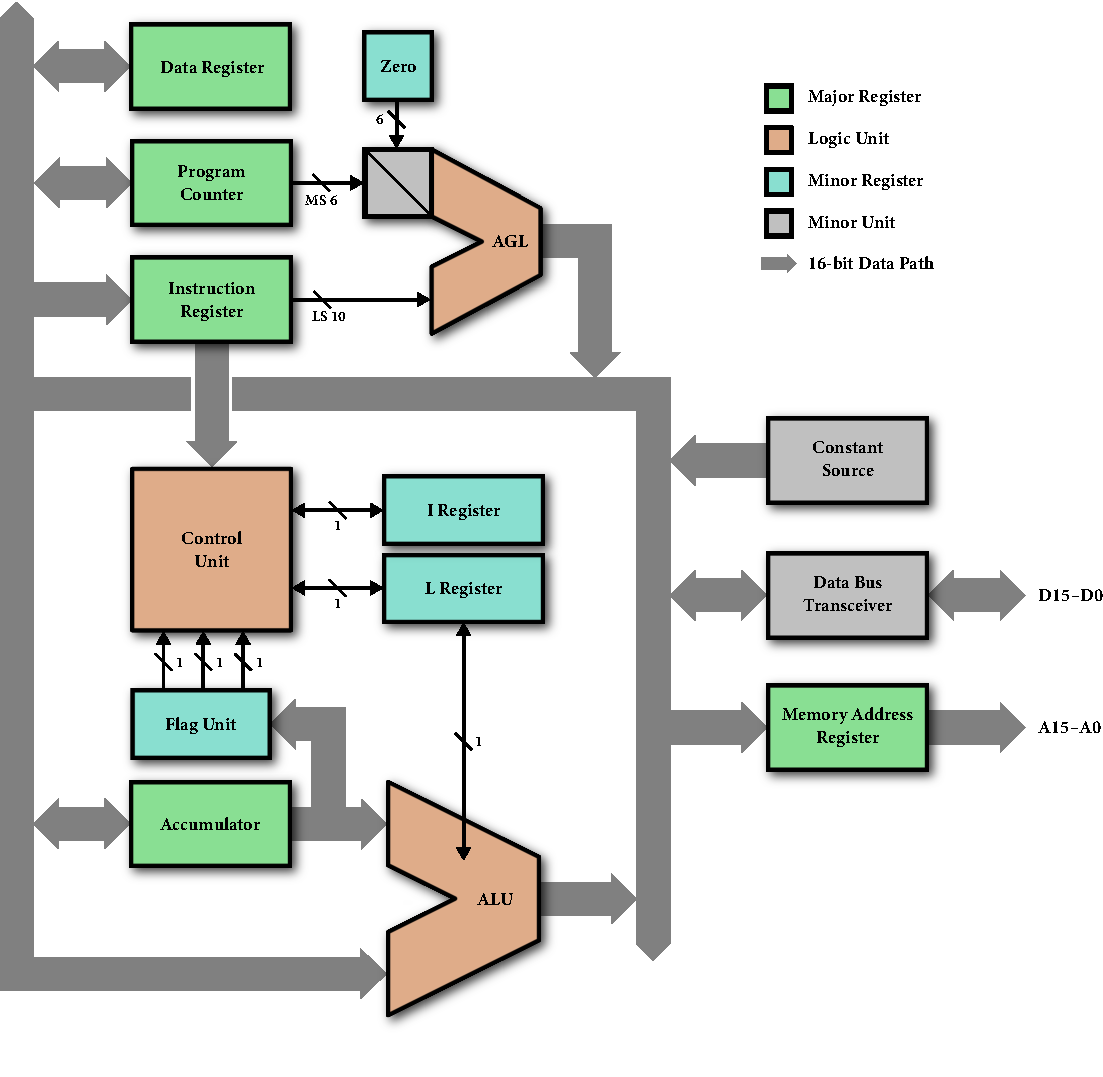
\includegraphics[width=\textwidth]{figs/datapath.pdf}\vspace{2em}\\
\end{figure*}

\end{document}

%%  LocalWords:  documentclass CFT Alexios PDP autoindexing Von LSI
%%  LocalWords:  Neumann microprograms microprogram microinstructions
%%  LocalWords:  et cetera kiloword KWord kilowords KWords Autoindex
%%  LocalWords:  SUBRET JSR TRAPRET ISRRET ISR autoindex th FC FFF tl
%%  LocalWords:  FFFF pagerel vlgrey linewidth fillstyle fillcolor de
%%  LocalWords:  addr FFFE IOT LIA JMP bitwise ORred asm bitfield CLA
%%  LocalWords:  CLL RBL RBR RNL RNR NOP linearc SNA SZA SSL SNN SNZ
%%  LocalWords:  SCL CLI STI SNP lll RET RTT SBL SBR SNL SNR TTY
%%  LocalWords:  disjuncted conjuncted ANDed
